\documentclass[12pt,a4paper,fleqn]{article}
\title{Progress Report}
\author{Syed Ahmad Raza}
\date{2016.12.15}
\usepackage{mathtools}
\usepackage{graphicx}
\usepackage{color}          % for color eps output
%\usepackage{layouts}       % for: \printinunitsof{in}\prntlen{\textwidth}

\begin{document}
\maketitle
\section*{Numerical solution for 1D heat transfer}
Forward time center in space (FTCS) method was used with the following formula:
\begin{equation}
T_i^{n+1} = T_i^n + \Delta t(\alpha \frac{\partial^2T}{\partial x^2})
\end{equation}

A time step of 0.001 was utilized. Grid independence tests were run at $t =
3500$ and grid independence was achieved at 158 intervals. The steady state was achieved at almost $t = 3000$.


\begin{figure}[p!]
\centering
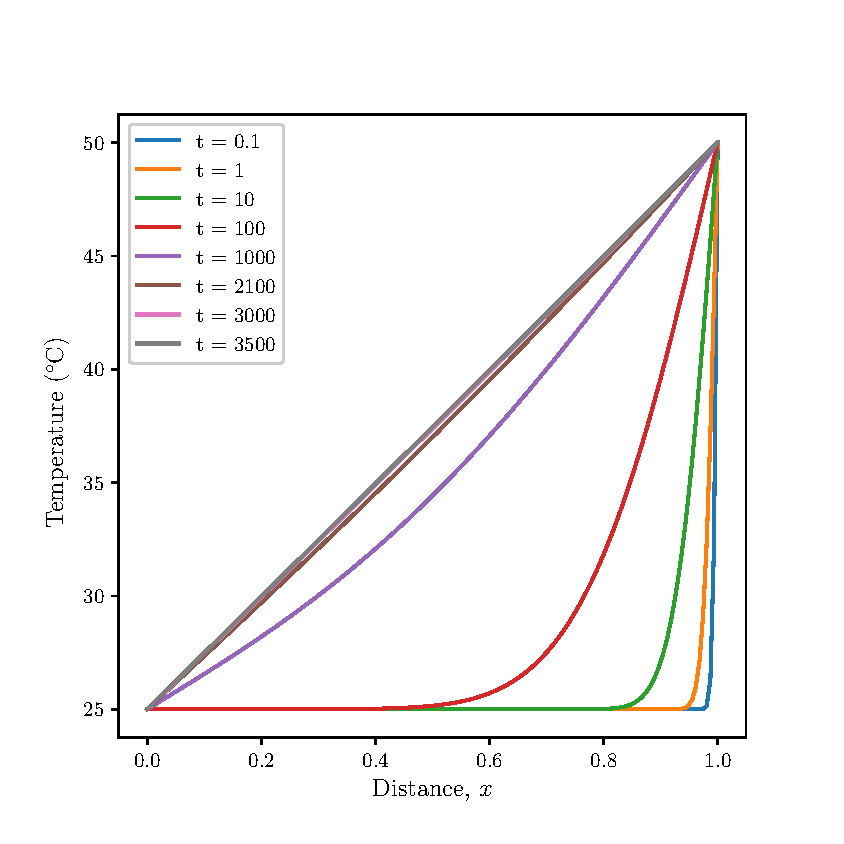
\includegraphics[width=\linewidth]{ht1dn158.eps}
\caption{Plot with 190 intervals and time step of 0.001 for various values of
time}
\end{figure}
\end{document}
